
Primero, lo que hicimos fue testear cuando se le pasaban muchos parámetros.

\begin{figure}[H]
\caption{Ejemplo de un lote de tareas con Task Consola}
\label{fig:ej71}
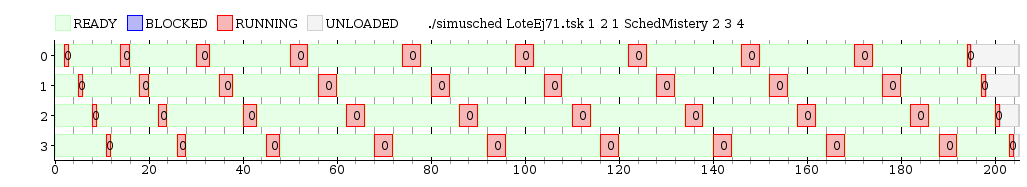
\includegraphics[width=1\textwidth]{imgs/ej7-1.png}
\end{figure}

Como se vé en la imagen, la cantidad de parámetros determina cuanto va a ser el quantum que se le asigna a cada tarea, progresivamente. Además gracias a este test, pudimos ver que hay preemption, y que el método probablemente sea similar a Round Robin.


Luego, lo que hicimos fue ver que pasa si una tarea se bloquea.

\begin{figure}[H]
\caption{Ejemplo de un lote de tareas con Task Consola}
\label{fig:ej72}
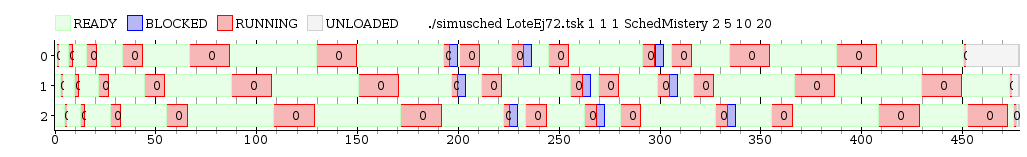
\includegraphics[width=1\textwidth]{imgs/ej7-2.png}
\end{figure}

Gracias a esta imagen pudimos confirmar que hay una idea de prioridades detrás de este scheduler. Esto se debe a que cuando una tarea se desbloquea, tiene \emph{más prioridad}, dado que por ejemplo, la tarea 0, despues de desbloquearse, se ejecuta antes que la tarea 2, que era la que a priori le tocaba, si se tratara de un Round Robin común y corriente.

Además, este test nos permitió ver que cuando una tarea se desbloquea va a la cola que le sigue en prioridad (de más prioridad).


Entonces, de esta manera confirmamos que se trata de un scheduling de prioridad, en el que hay $n$ colas (si nos pasaron $n-1$ parámetros), donde cada cola tiene un quantum igual al parámetro que corresponde (o 1 si es la primera). Y lo que hace el algoritmo es ir por la lista de colas buscando alguna cola no vacía, y si encuentra alguna no vacía corre la próxima tarea que corresponda.

Además, cuando una tarea es desalojada, pasa a estar en la cola siguiente (de menor prioridad) que la que estaba antes, y si estaba en la de menos prioridad se queda en esa.

En cuanto a la implementación, tenemos un vector de colas, y un vector de quantums (cuanto es el quantum de cada cola de tareas). Además, tenemos un entero que nos indica cuanto tiempo le queda a la tarea actual y de que cola salió.

Entonces, cuando cargamos una tarea la ponemos en la cola mas prioritaria. Cuando una tarea se desbloquea, la ponemos en la cola anterior (de más prioridad). Cuando una tarea debe ser desalojada porque se acabó el tiempo que se le asignó, se recorre el vector de colas buscando la primera no vacía y en caso de que la encuentre, popea un pid y lo pone a correr. En caso de que no encuentre, continúa corriendo la tarea actual.

